\chapter{部分可见积木世界构建方法}
\label{dataset}
本章提出一种基于ASP的部分可见积木世界构建方法(ASP-Based Block World Generation,简称ABWG),
旨在实现具有可控空间关系的部分可见积木世界图像的即时生成,
并据此构建空间推理问答数据集POVQAD,以支持对本文所提出的神经符号VQA框架进行系统评估。
具体内容将围绕以下三方面展开:部分可见积木世界构建任务说明、基于ASP的图像生成方法,以及POVQAD数据集的构建过程。
\section{部分可见积木世界构建任务说明}
部分可见积木世界的构建任务包括两个方面:一是根据用户发出的自然语言指令,即时生成具有指定的空间关系的部分可见积木世界图像
;二是构建空间推理问答数据集POVQAD。

前者在自动规划课程的教学中具有重要的实际意义。积木世界作为该领域中经典的教学与研究场景,
教师往往需通过控制积木间的空间布局,构造具备多样初始状态的任务场景,用以测试和演示不同规划算法的表现。
为此,自动规划教学系统亟需具备根据用户自然语言描述实时生成满足语义约束的积木世界图像的能力,并支持围绕图像进行空间关系相关的视觉问答。
因此,设计一种能够根据约束自动生成图像的机制,是推动自动规划教学智能化、交互化发展的关键一步。

构建数据集POVQAD的目的是克服现有模拟积木世界视觉问答数据集CLEVR所存在的若干局限性,具体包括以下三点:
\begin{enumerate}[nosep]
\item 场景信息完全可见。 在CLEVR数据集中,图像中的所有对象都是完全可见的,问题涉及的实体均能直接观察。这种设定无法模拟现实世界中“部分可见”的复杂场景,限制了模型在不完整感知条件下进行推理的能力。例如,对于问题 “What color is the cylinder to the left of the red sphere?”,图像中左侧明确可见一个蓝色圆柱体,右侧是红色球体。模型只需定位球体并查找其左侧物体即可直接得出答案,无需更复杂的场景理解或假设补全。
\item 缺乏环境级逻辑约束。 CLEVR中的场景未设定必须满足的背景约束,例如“所有红色物体必须是立方体”之类的规则缺失,使得推理任务缺乏结构性和复杂性,难以考察模型结合显式知识进行深度推理的能力。例如,在回答“Are there more cubes than red things?”时,模型只需简单计数即可给出答案,根本无需考虑隐藏规则或类属约束。
\item 不涉及空间推理。 CLEVR仅将空间关系作为辅助手段,用于建立目标物体与参照物体之间的相对位置关系,并不真正探讨位置本身。例如,它不会直接提出“某物体位于哪个位置”或“两个物体的空间关系如何”这类问题。因此,该数据集在空间推理方面存在明显缺失。
\end{enumerate}

下面将介绍部分可见积木世界的基本设定,为后续基于ASP的方法实现图像生成与POVQAD数据集构建提供概念基础与语义框架。
\subsection{部分可见积木世界的定义}
积木世界是一种由多个形状、颜色、大小各异的物体构成的图像世界,
这些物体以离散方式摆放在三维空间内,并满足一定的空间布局规则。该世界的状态通常具有良好的结构性与可控性,便于形式逻辑建模与基于规则的推理。

下面本节从积木世界的基本组成、约束模板两方面对部分可见积木世界的定义展开介绍。
\subsubsection{积木世界基本组成}
积木世界的基本组成可从以下三个主要维度进行描述:
\begin{enumerate}[nosep]
\item 物体属性。 每个积木被视为一个具备静态属性的独立个体,主要包括以下四类属性:
\begin{enumerate}[nosep]
\item 形状:立方体、球体、圆柱体、圆锥体;
\item 颜色:红色、蓝色、绿色、黄色、灰色、棕色、紫色、青色;
\item 尺寸:小、中、大;
\item 材质:橡胶、金属。
\end{enumerate}
这四种属性既是物体最直观、易区分的感知特征,也与CLEVR数据集保持一致,便于后续的比较研究。
对每类属性的取值范围加以限定(如颜色八种、形状四种、材质两种、尺寸三种),有助于控制推理复杂度与答案搜索空间,避免组合过多带来的计算负担。
\item 空间关系。本文对图像中物体之间的空间关系,选取了上、下、前、后、左、右这六种基本方向关系作为研究对象,这一设计具有以下几点合理性:
\begin{enumerate}[nosep]
\item 语义基础性强,覆盖主流空间语言表达。
这六个方向关系与人类空间认知中的基本坐标轴(x、y、z)紧密对应,构成了绝大多数空间描述中的基础语义单元。
它们不仅是自然语言中空间关系的核心词汇(如“在左边的红色球体”),也是几何推理中最基本的参照方向。
通过组合这六种关系,可以表达复杂位置结构而无需引入冗余关系。
\item 结构可控性强,便于形式化建模与推理。
选择有限的六类方向关系,有助于控制逻辑建模复杂度,避免因冗余或模糊的空间词(如“斜对角”“近旁”)引入不确定性。
每种关系均可通过规则明确定义(例如通过坐标或投影判断),保证推理结果的一致性和可验证性。
\item 支持三维推理,满足立体场景建模需要。
相较于只在二维平面上定义“上下左右”,引入“前后”关系使模型具备三维推理能力,更贴合真实或拟真场景下的空间认知需求。
尤其在积木遮挡问题中,前后关系对于判断可见性与空间遮挡至关重要。
\end{enumerate}
\item 区域划分。本文对图像中的空间进行划分,形成四个区域,区域编号取值分别为0、1、2、3,并同时规定每个物体只能在图像的一个区域中,不能同时跨多个区域。
为图像空间划分区域,主要的优势在于为图像生成和问题生成指定作用范围约束,有利于可控地提升数据集的复杂性和多样性。
\end{enumerate}
\subsubsection{部分可见性}
在VQA领域,部分可见性指的是在观察场景时,图像中的部分信息由于遮挡、视角限制或场景复杂性而不可直接获得的情况。
与理想的全可见环境相比,部分可见性更符合真实世界的感知条件,也对模型的空间推理与信息补全能力提出了更高要求。
近年来,越来越多研究关注如何在部分可见的场景下完成问答任务,以增强模型在实际应用中的鲁棒性与泛化能力。

在本文所构建的积木世界场景中将部分可见性从两个维度进行定义,即部分可见场景和不可见场景。二者的主要区别在于:部分可见场景中,
仍可以从图像中感知到被遮挡物体的一些特征;不可见场景中,被遮挡物体完全被其它物体遮挡,无法从图像中直接感知到被遮挡物体的任何特征。

部分可见场景是一种“背景知识不足,且图像中待查询物体被部分遮挡”的情形,这种情形代表了多数实际视觉任务中遇到的问题:
视觉系统可以检测部分被遮挡的物体,但缺乏对完整结构的观测,
难以仅靠视觉识别完成推理任务。本研究设计此类情境,旨在展示无需额外标注或监督,仅通过空间逻辑推理即可提升问答系统表现。
如图\ref{fig:partial-observable-scene-example}所示,仅凭视觉感知无法直接回答问题“球体是否在立方体的左侧?”,
但结合已有空间规则与遮挡顺序,系统可准确判断相对位置关系。这类问题强调了空间逻辑推理在提升弱监督视觉问答中的作用。
\begin{figure}[h]
\centering
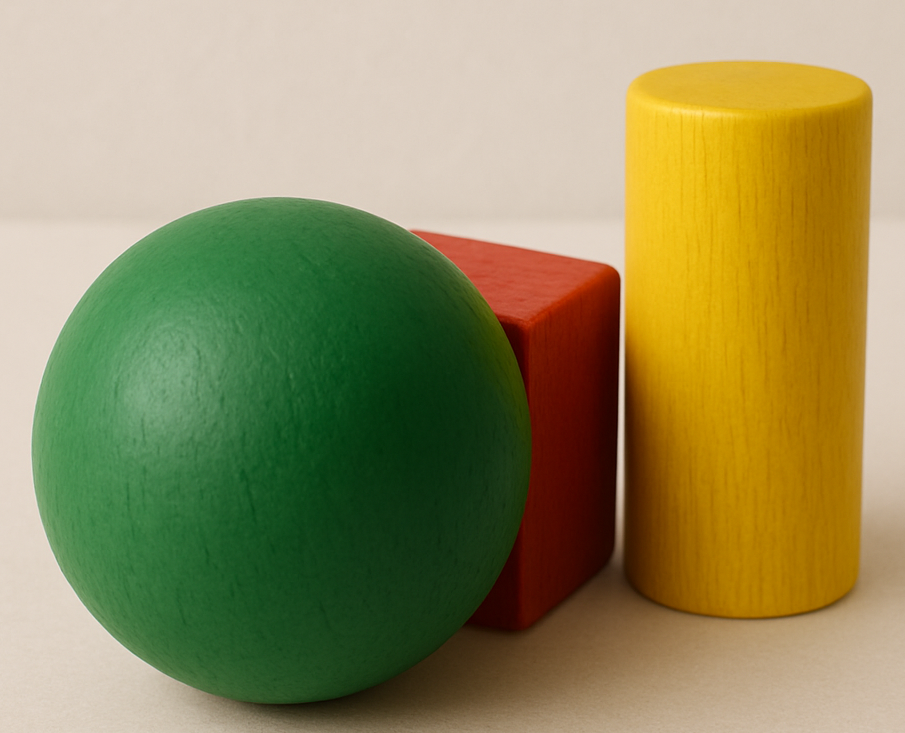
\includegraphics[scale=0.25]{figures/部分可见场景示例.png}
\caption{部分可见场景示例}
\label{fig:partial-observable-scene-example}
\end{figure}

不可见场景是一种“背景知识中已知,但图像中不可见”的情形。
此类情形中,某些物体或其属性未出现在图像中,但依据环境布置的规则或先验知识,推理系统应当具备“补全”或“外推”能力。
如图\ref{fig:not-observable-scene-example}所示,该图片的背景约束信息是:“场景中所有蓝色球体都放置在红色圆柱体后面,且每个红色圆柱体后面恰好有一个蓝球。”,
提问的问题是:“该图像中有几个蓝色球体?”。尽管视觉输入中没有检测到任何蓝球,但根据背景规则和红色圆柱体的数量,
系统应能得出“存在两个蓝球”的结论。这类问题强调的是利用背景知识进行结构性空间推理。
\begin{figure}[h]
\centering
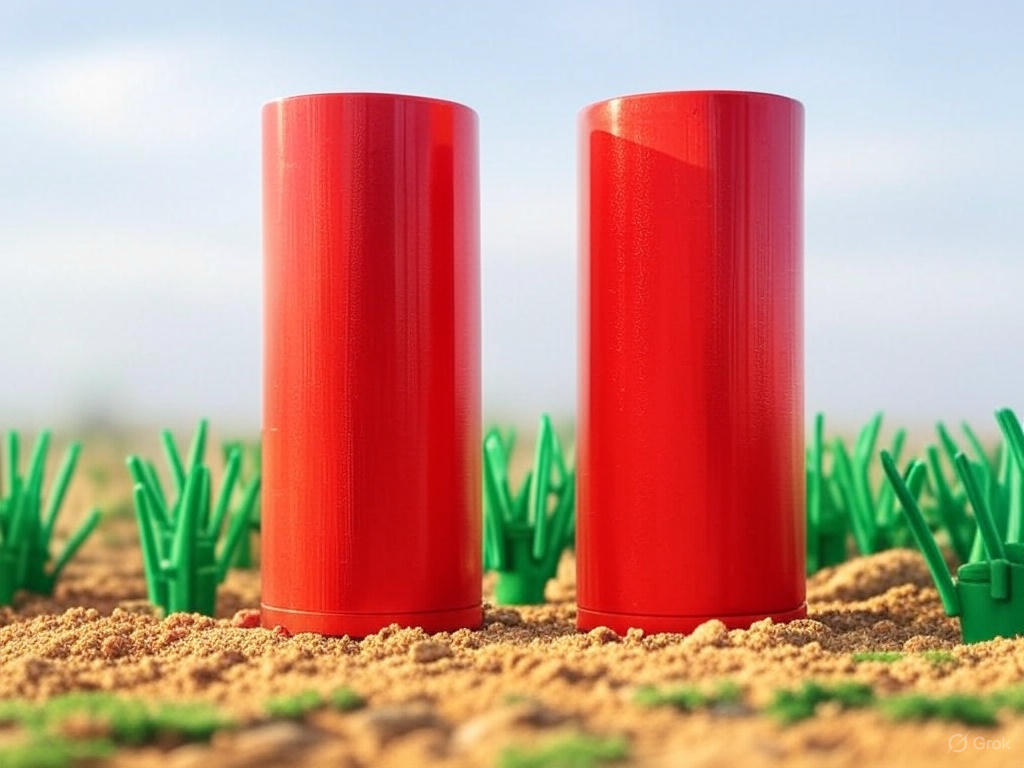
\includegraphics[scale=0.16]{figures/不可见场景示例.jpg}
\caption{不可见场景示例}
\label{fig:not-observable-scene-example}
\end{figure}

在具体实现上,本文使用遮挡面积比例和遮挡关系来控制这些遮挡情形的生成。当遮挡面积比例为1时,表明两个物体构成的是
完全遮挡关系;当遮挡面积比例大于0小于1时,表明两个物体构成的是部分遮挡关系。
\subsection{约束模板}
\label{constraint-template}
约束模板是抽象定义的一类通用规则形式,这些规则可以通过填入特定参数(例如区域、属性、属性值、数量等)
来实例化为具体约束,从而用于生成符合特定空间关系、区域分布或者属性限制的积木世界图像。

将约束模板引入临机生成可控空间关系的部分可见积木世界的构建中,出于以下几方面的考量:
\begin{enumerate}[nosep]
\item 保证场景的逻辑一致性。约束模板在构造场景时充当“规则”,确保生成的每个场景都遵循设定的逻辑和规律,
例如“一个区域不能有超过 3 个大物体”或“同一区域中不允许出现两个相同材质的物体”。这有助于构建符合特定认知与推理需求的合理场景。
\item 可复用、结构清晰、易于扩展。模板化的设计使得规则可以模块化、参数化、重复使用,便于添加新规则或调整已有规则。
例如要增加“区域之间不能有相同材质的物体”,只需添加一条模板,不需要重写整个生成逻辑。
\item 支撑任务复杂度的调控。通过对模板赋予不同的参数,生成不同的约束,以及约束之间的各种组合,可以人为控制
任务难度和积木世界的复杂度。
\item 提升部分可见积木世界的多样性和可控性。通过预先设计一系列模板,可以系统地控制场景多样性
(如属性组合、空间关系、数量限制)而不是随机生成。这种可控性有助于评估模型对不同类型推理问题的能力。
\end{enumerate}

在约束模板的设计上,本文针对部分遮挡和完全遮挡两种情况,设计了约束模板,并以ASP形式给出。
使用ASP来进行表示的原因在于,ASP 是一种声明式逻辑编程语言,特别擅长用于描述约束、规则、组合问题,通过使用 ASP,可以形式化地定义物体属性、数量、空间关系等复杂逻辑要求。
以下为部分约束模板示例,所有的约束模板在附录\ref{appendix:constraints}中予以展示。
\begin{enumerate}[nosep]
\item 遮挡关系的物体对数不少于N。
\begin{lstlisting}
:- #count{X,Y : occludes(X,Y), obj(X), obj(Y)} < N.
\end{lstlisting}
\texttt{\#count}是一种聚合操作符,用于计算满足某个条件的项的数量。
\texttt{:-}和\texttt{< N}共同表示遮挡关系数量少于N就违反约束,所以能够保留下来的都是遮挡关系数量至少为N的答案集。
另外\texttt{occludes(X,Y)}谓词表示物体X和物体Y之间存在遮挡关系,且X是遮挡物体,Y是被遮挡物体;
\texttt{obj(X)}和\texttt{obj(Y)}分别表示X和Y都是对象。
\item 每个被遮挡物体的遮挡率不超过R'。
\begin{lstlisting}
:- occlusion_rate(T, R0), R0 > R_prime.
\end{lstlisting}
其中\texttt{occlusion\_rate(T, R0)}谓词表示物体T为被遮挡物体,且T的被遮挡面积所占比例为R0。另外,此处使用R\_prime表示R'。
由于这是一个ASP约束,不能通过约束的是R0大于R'的答案集,所以剩余有效的答案集,R0均小于等于R'。
\item 区域R中的物体最多有N个。
\begin{lstlisting}
:- #count{X: obj(X), at(X,R)} > N.
\end{lstlisting}
谓词\texttt{at(X,R)}用于表示 X 在区域 R。这一约束可用于控制一个区域或者整个积木世界中最多放置多少个物体。
\item 场景中至少有K对物体呈现“左-右”相邻的空间关系。
\begin{lstlisting}
:- #count{X,Y: left(X,Y), obj(X), obj(Y)} < K.
\end{lstlisting}
\texttt{obj(X)}和\texttt{obj(X)}用于表示X和Y都是合法对象,\texttt{left(X,Y)}表示X在Y的左侧。
\texttt{< K}表示这些 (X,Y) 对的总数少于 K。
\texttt{:-}表明这是一个约束,意思是:如果这个条件为真(即遮挡对少于 K),则这个答案集被判定为非法。
\item 目标物体的左侧有且只有L个物体。
\begin{lstlisting}
:- #count{X: left(X,T), obj(X)} != L.
\end{lstlisting}
\texttt{\#count}作为聚合操作符,用于计算满足某个条件的项的数量,\texttt{left(X,T)}表示对象X在对象T的左边,
\texttt{obj(X)}用于声明X是一个合法的对象。\texttt{:-}表明该语句为一个约束,意思是:如果这个条件为真(即数量不等于 L),那么该答案集 不合法,会被 ASP 系统丢弃。
故最终所得的答案集中都是目标物体T的左侧恰好有L个物体的情况。
\end{enumerate}
\subsection{根据约束构建部分可见积木世界}
获得约束规则后,仍需要进行一系列流程方能获得部分可见积木世界图像。下面在此对后续流程进行简要介绍,具体的实现细节因构建任务
的不同而略有差异,将分别在3.2节基于ASP的部分可见积木世界的构建和3.3节POVQAD数据集构建中分别予以介绍。
\begin{enumerate}[nosep]
\item 生成环境。在获得具体约束规则之后,需要进一步生成环境。
环境是根据若干条约束规则生成的,表示部分可见积木世界必须遵守的一系列限制条件。
在具体流程上,需要将全局约束与获得的具体约束规则进行组合,共同输入ASP求解器进行求解。若能正常执行并获得至少一个答案集,
则表明获得的具体约束规则之间没有出现逻辑冲突的情况,可以获得环境,后续可以据此生成部分可见积木世界图像。若执行报错或者答案集为空,
则表明不能获得环境,停止进行后续进一步的流程。全局约束是所有环境都应遵循的约束,对整个积木世界进行了基本定义,
例如“平面区域划分为4个,编号0、1、2、3。”就是通过全局约束定义的,
ASP形式为\texttt{region(0). region(1). region(2). region(3).}。
本文所用的所有全局约束在附录\ref{appendix:environment}予以了展示。
\item 构建场景。场景是一个具体的实例化结果,描述了一个满足环境的要求的积木世界布局,包括了积木世界中所有对象的属性、
位置及其相互空间关系、图像等等。场景是环境的具体化,与图像和关于图像的问题生成直接相关。在生成场景的过程中,需要依据完整场景图进行进一步的生成。
完整场景图中包括了所有对象的属性。

构建场景的大致流程如下:首先将环境输入ASP求解器进行求解,获得满足环境的答案集,此处一个答案集对应一个完整场景图。
随后,根据实际需要,生成部分可见场景图(部分遮挡的情形)和不可见场景图(完全遮挡的情形),以供后续生成图像使用。
部分可见场景图和不可见场景图分别对应部分可见场景和不可见场景,此时已经基本完成两种场景的生成,但仍缺少图像信息,需要
生成图像环节进行进一步的处理。
\item 生成图像。基于部分可见场景图和不可见场景图,使用Blender进行渲染生成图像,并完善前一步中生成的基本完整的场景,获得最终的
部分可见场景和不可见场景。
\end{enumerate}

本章后续的基于ASP的部分可见积木世界的构建和POVQAD数据集构建,都将大致按照上述流程进行,最终获得部分可见积木世界的图像。
\section{基于ASP的部分可见积木世界构建方法}
\subsection{构建目标与技术选型}
构建基于ASP的部分可见积木世界的总目标为:LLM能够根据用户(例如参与自动规划课的教师或者学生)提供的以自然语言形式描述的对积木世界中物体属性、遮挡关系
等方面的要求,生成具体的以ASP形式描述的约束规则,后续基于该组约束规则生成部分可见积木世界图像。
基于这一总目标,本文决定采用提示学习的方法,
使用DSPy作为提示管理与语义生成框架,让LLM习得预定义的约束模板中的深层语义,使其掌握如何根据用户要求进行对应的ASP约束规则生成。
选择基于ASP来构建部分可见积木世界,有以下几点原因:
\begin{enumerate}[nosep]
\item ASP具有明确的逻辑语义和出色的可解释性,能够对积木世界中关于位置、遮挡、颜色、堆叠关系等复杂规则进行形式化建模,同时保证生成图像的语义一致性和规则可追溯性。
\item ASP支持非单调逻辑和默认推理,能够自然处理部分可见场景中关于不确定信息的表达,如“某个物体可能被遮挡”或“在未观察到的情况下推测其存在”,这一特性恰好契合本文数据集所需建模的现实感知不完全性。
\item ASP具备高效的求解器(如 Clingo),能够在大规模规则集合下快速生成满足约束的实例,便于数据集大批量合成。
\end{enumerate}
而选择采用对LLM进行提示学习的方法,并使用DSPy来实现提示学习,出于以下几点考量:
\begin{enumerate}[nosep]
\item LLM在经过精心设计的提示引导下,能够在无需额外训练的条件下,对自然语言进行结构化转换,自动生成语法正确且语义准确的ASP规则,从而大幅降低规则生成的门槛,实现自然语言到形式化逻辑的高效映射。
\item 提示学习方法具有更强的灵活性和泛化能力。传统的数据驱动方法往往需要大量标注好的场景-约束对以训练一个专用模型,而这在积木世界中高维组合空间下代价极高且难以穷尽所有规则变体。相比之下,提示学习方式可通过少量示例演示(in-context learning)来引导LLM快速适应特定风格的规则生成任务,有效降低训练样本依赖,提升低资源条件下的数据生成效率。
\item DSPy 支持以声明式模块化方式组织提示,通过将任务划分为结构清晰的子模块(如信息提取、格式转换、规则生成等),能够更好地管理提示的复杂性与多样性。这一特性对于本任务中“从自然语言描述到ASP规则生成”的流程尤为重要,因其涉及多个阶段的信息加工与转换过程,DSPy提供的模块组合与链式执行机制(Chain of Prompts)有助于确保生成过程的逻辑一致性和中间步骤可控性。
\item DSPy 框架原生支持 与大语言模型的集成和输出约束,包括结构化输出格式、示例演示(少样本 prompting)、多候选响应重排序(reranking)等机制。对于本任务而言,ASP规则具有严格的语法与逻辑要求,DSPy 提供的 Signature 接口允许精确定义输入-输出格式,使生成的规则更符合目标结构。同时,它还支持在候选结果中选择最优输出,提升了ASP规则生成的正确率与稳定性。
\item DSPy 支持与评估指标联动的“自我改进”机制,可在一定程度上对提示进行自动优化,从而提升生成结果质量。
\end{enumerate}

以下将对构建流程展开介绍。
\subsection{构建流程}
构建流程图如\ref{fig:asp-based-block-world-construction}所示。首先使用\ref{constraint-template}中预定义的模板
构建提示词,对LLM进行提示学习。此后,LLM根据输入的以自然语言描述的部分可见积木世界生成指令,生成具体约束,再由具体约束生成环境。
此后,根据环境生成部分遮挡场景或完全遮挡场景,最后Blender根据场景渲染得到符合约束要求的部分可见积木世界图像。
\begin{figure}[h]
\centering
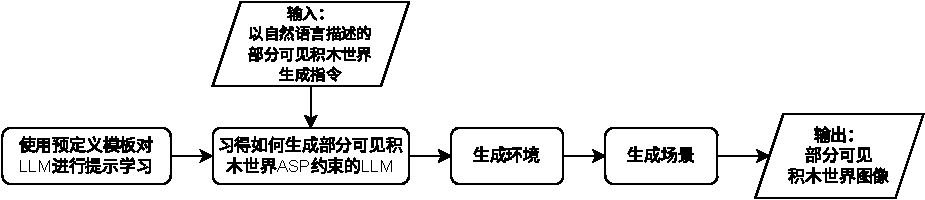
\includegraphics{figures/asp-based-block-world-construction-crop.pdf}
\caption{基于ASP的部分可见积木世界构建流程}
\label{fig:asp-based-block-world-construction}
\end{figure}
\subsubsection{LLM生成约束}
\label{self-define-func}
\begin{enumerate}[nosep]
\item 任务定义。
DSPy是一个面向语言任务的程序性提示框架,能够在具备结构化的输入输出约束的前提下,
调用LLM完成特定子任务。在本任务中,将“自然语言描述的部分可见积木世界应满足的约束规则$\rightarrow$以ASP表示的部分可见积木世界的约束规则”建模为一个标准的DSPy模块。在实现上,通过DSPy的\texttt{Signature}定义任务结构,其中明确了模块的目标,即根据用户输入的部分可见积木世界应满足的约束规则生成其对应的ASP表示。
\begin{lstlisting}
class ParseQuestionToASP(Signature):
    question = DSPy.InputField(desc="自然语言描述的部分可见积木世界应满足的约束规则")
    asp_code = DSPy.OutputField(desc="以ASP表示的部分可见积木世界的约束规则")
\end{lstlisting}
\item 提示词设计。
本节基于已设计的约束模板设计提示词,要求LLM学习如何根据以自然语言形式描述的部分可见积木世界限制条件
生成对应的ASP规则。以下为部分提示词的示例:
\begin{lstlisting}
下面将提供给你几组以自然语言描述的对部分可见积木世界的限制条件,以及各个限制条件对应的以ASP形式表示的约束,请你学习如何根据自然语言生成这些ASP形式的约束。
在后续的对话中,将会向你发送一系列自然语言描述,需要你分别以ASP形式进行表示。

自然语言描述:遮挡关系的物体对数不少于N。
ASP规则::- #count{X,Y : occludes(X,Y), obj(X), obj(Y)} < N.

自然语言描述:每个被遮挡物体的遮挡率不超过R'。
ASP规则::- occlusion_rate(T, R0), R0 > R_prime.

自然语言描述:区域R中的物体最多有N个。
ASP规则::- #count{X: obj(X), at(X,R)} > N.

自然语言描述:场景中至少有K对物体呈现“左-右”相邻的空间关系。
ASP规则::- #count{X,Y: left(X,Y), obj(X), obj(Y)} < K.

自然语言描述:目标物体的左侧有且只有L个物体。
ASP规则::- #count{X: left(X,T), obj(X)} != L.
\end{lstlisting}
\item 提示词优化。
为进一步提升提示学习的效果,提升生成描述部分可见积木世界的ASP约束的准确率,本文在此引入验证集驱动的提示优化策略。本文设计了另一组同类的约束模板组成验证集,通过
生成ASP约束的语法正确率和语义正确率对少样本示例顺序与提示模板进行自动调整。
语法是否正确的判断标准是:ASP程序输入Clingo后,如果能够正常执行,不提示错误,则视为语法正确,否则视为语法错误。
语义是否正确的判断标准是:要求LLM根据验证集中以自然语言描述的对部分可见积木世界的约束,来生成对应的ASP程序。
此后将生成的ASP程序经Clingo获得的执行结果和验证集中自然语言描述对应的约束经Clingo执行的结果进行比较。
如果两者的执行结果一致,则可认为语义正确,否则认为语义错误。
此处采用 DSPy 提供的 BootstrappedFewShotOptimizer 优化器,以生成的 ASP 约束的语法正确率和语义正确率作为评价指标,训练优化提示内容。
选择 BootstrappedFewShotOptimizer 优化器主要基于以下几点考量:
\begin{enumerate}[nosep]
\item 与结构化问答任务不同,用户描述的约束常常具有多种表达方式
(如“不能出现红色球体”“区域1不应有红球”等语义等价描述)。BootstrapFewShotOptimizer 
能够通过自举式学习不断挖掘多样示例,提升提示对自然语言语义变体的适应能力。
\item 本任务的输出为 ASP 形式的逻辑规则,具备明确结构与语法约束。该优化器具备结构保持能力,
能稳定生成语法正确、模板匹配度高的 ASP 表达式,从而保证数据质量。
\item 在样本数量有限的前提下,该优化器能基于已有示例动态构造 少样本 提示组,降低对大规模人工标注的依赖,显著减少模板调试成本。
\item BootstrapFewShotOptimizer 支持通过自定义评估函数对生成结果进行语义检查,从而形成闭环优化机制,提升生成质量。
\item 优化后的提示不仅适用于当前任务,还可迁移到其他类似的规则抽取任务中(如空间约束生成、场景逻辑分析等),为后续研究提供通用工具基础。
\end{enumerate}

优化器中的自定义评价函数在此处记为\texttt{ValidScore},用于判断LLM输出的ASP约束规则是否满足语法正确和语义正确。下面对如何定义并计算自定义评价函数的值给出相关解释:

对于一个程序$P$,Clingo用于计算该程序的答案集。
进而该过程可以等价于:定义一个函数$f(P) = AS(P)$,其中$AS(P)$表示程序P的所有回答集(可能为空)。
LLM根据提示$x$生成的ASP程序,记为$y ~ P_L(|x)$。与$x$对应的能够真实表示问题的标准ASP程序,记为$y^*$。按照以下步骤来进行验证:
首先基于$x$构建一个表示具体实例的事实集$F_{y^*}$。接着,构造两个完整的ASP程序:
\begin{enumerate}[nosep]
\item $P = y \cup F_{y^*}$:由模型生成程序与事实集合成的程序。
\item $P^* = y^* \cup F_{y^*}$:由标准程序与事实集合成的程序。
\end{enumerate}

此后,执行以下评估步骤:
\begin{enumerate}[nosep]
\item 语法检查。该步骤的执行结果记作$syntax$。调用Clingo运行程序$P$,若未发生解析错误,则认为模型生成的程序 $y$ 在语法上是正确的,则判定为语法命中,记$syntax = 1$。否则,则判定为不命中,记$syntax = 0$。
\item 语义检查。该步骤的执行结果记作$semantic$。分别用 Clingo 计算$f(P)$与$f(P^*)$,分别得到各自的答案集$AS(P)$与$AS(P^*)$。若$AS(P)$与$AS(P^*)$完全匹配,则判定为语义命中,记$semantic = 1$。
否则,则判定为不命中,记$semantic = 0$。
\end{enumerate}

则根据上述评估步骤,可给出自定义评价函数的数学定义:
$$ValidScore = syntax \land semantic $$
\item 输出。
经过优化后的提示模块,能够将输入的以自然语言描述的对部分可见积木世界的约束,准确地转换为ASP规则。
后续向LLM输入以自然语言描述的部分可见积木世界生成指令,即可得到以ASP表示的部分可见积木世界约束。
例如,针对输入“积木世界的所有物体之间,最多有4对‘前-后’空间关系”,LLM最终输出示例如下:
\begin{lstlisting}
:- #count{X,Y: front(X,Y), obj(X), obj(Y)} < K.
\end{lstlisting}
生成的ASP规则在后续将用于环境的生成,为部分可见积木世界数据集的生成奠定坚实基础。
\end{enumerate}
\subsubsection{生成环境}
环境是根据若干条约束规则生成的,表示部分可见积木世界必须遵守的一系列限制条件。
在基于ASP的部分可见积木世界构建中,环境即“用户以自然语言描述的生成指令在经过LLM处理后生成的基于ASP的约束规则与全局约束规则,两者
共同输入ASP求解器后所得的答案集”。

那么在生成环境时,将全局约束规则与LLM生成的约束规则进行拼接,形成完整ASP程序,并由Clingo对ASP程序进行求解。
如果Clingo的输出至少存在一个答案集,说明当前约束可满足,将所得结果(即环境)保存到ASP程序的\texttt{.lp}文件中。
如果Clingo没有答案集,说明当前约束不满足(unsatisfiable),不再继续进行部分可见积木世界的生成。
\subsubsection{构建场景}
场景是基于环境的基础上进一步生成而得。将环境的\texttt{.lp}文件输入Clingo进行求解,得到若干个答案集。
此后,对答案集进行解析,以获得完整场景图。对答案集进行解析的过程实际上是对谓词进行解析的过程,主要\texttt{has\_property}和\texttt{at}两个谓词进行解析,
最终形成以JSON格式存储的场景图。

随后,检查答案集中是否存在部分遮挡约束(以谓词\texttt{occludes}和谓词\texttt{occlusion\_rate}共同表示,且遮挡面积比例大于0小于1的情况)
、完全遮挡约束(以谓词\texttt{occludes}和谓词\texttt{occlusion\_rate}共同表示,且遮挡面积比例等于1的情况)。
如果存在,则分情况进行如下操作:
\begin{enumerate}[nosep]
\item 部分遮挡(\texttt{occlusion\_rate}中遮挡面积比例$0 < R < 1$):在原有的完整场景图的基础上,添加occlusion字段的信息,例如:
\begin{lstlisting}
{
  "occlusion": [
    {0, 1, 0.3}
  ]
}
\end{lstlisting}
occlusion字段中,每个三元组都表示一对遮挡关系。其中第一个表示被遮挡物体的编号,第二个表示遮挡物体的编号,编号均与完整场景图的objects
中的物体编号保持一致。其次,遮挡面积比例$R$作为三元组的第三个数据项。在后续Blender根据场景图渲染生成积木世界图像时,将会
将两个物体按照指定的遮挡面积比例和被遮挡关系进行生成。此时所得的场景图为部分可见场景图。
\item 完全遮挡(\texttt{occlusion\_rate}中遮挡面积比例$R = 1$):在原有完整场景图的基础上,将\texttt{occludes}中的
被遮挡对象(即谓词中的第一个物体)的相关信息从完整场景图的objects字段中进行删除,以模拟完全遮挡发生时,图像中无法直接感知到任何信息的情况。
此时所得的场景图为不可见场景图。
\end{enumerate}
经过以上谓词解析的过程,得到部分可见场景或者不可见场景,以便后续Blender进行渲染生成图像。
\subsubsection{生成图像}
\label{image-generation}
生成图像的目的是:根据前一步生成的基本完整的场景中的物体信息,使用Blender进行渲染,最终生成部分可见积木世界图像。
具体包括如下环节:
\begin{enumerate}[nosep]
\item 初始化Blender渲染对象。在这一步中,主要是设置一系列渲染参数,包括分辨率、GPU设置等等。
\item 定义场景字典。该字典中保存了场景的元信息(即将生成的图片名称等)、物体信息和方向信息。
\item 方向向量计算。先获取在场景初始化时添加的平面的法向量,此后计算摄像机的方向向量,并将
摄像机的方向向量投影到平面上,得到相对于平面的方向向量。计算完成之后,将平面删除,避免影响后续渲染。
\item 向场景中添加物体。根据场景图中的物体信息,将物体添加到场景中。
在生成部分可见场景的图像时,要注意根据\texttt{occlusion}字段中各个三元组提供的遮挡关系,来生成遮挡的情形。
\item 计算物体之间关系。基于物体的三维坐标和场景的方向向量,遍历场景中的每对物体,
计算得出空间中上、下、左、右、前、后等关系。判断两个物体之间是否存在某种关系的阈值设置为0.2,即如果两个物体之间的
方向向量的点积大于0.2,那么认为它们具有该关系。阈值可以自定义进行修改。
\end{enumerate}

\subsection{转化正确率实验}
本实验的目的为:验证本文提出的基于ASP的部分可见积木世界构建方法中,经过提示学习后的LLM将自然语言的积木世界生成指令转化为对应约束的准确率。

本实验采用两种实验方法,方法一中采用对没有学习过预定义约束模板的LLM直接下达生成部分可见积木世界的ASP约束的指令,方法二中对前述经过提示学习后的LLM输入生成部分可见积木世界的ASP约束的指令。
通过两种方法的生成准确率的对比,可以证明本章设计的预定义约束模板和提示策略的有效性。

实验数据集采用构造的另一组“自然语言描述的积木世界生成指令-ASP约束规则”作为测试集,记为$T$。$T$中所有样例按照本文设计约束模板
进行生成,每种模板在$T$中的数量占比做到均衡分布,避免出现偏态分布的情况。实验过程中,将自然语言描述的积木世界生成指令作为输入,
对LLM生成结果与$T$中对应的ASP约束规则这两者之间做语法检查和语义检查,计算在三种不同LLM上,前述两种方法在数据集$T$上的语法正确率和语义正确率。

考核指标选取语法正确率和语义正确率,在前文已有定义,此处不再赘述。实验环境的配置方面,CPU为Intel Core i9 12900K,内存为128GB,显卡为2张Nvidia RTX4090。
另外在实验过程中,对实验重复进行5次,以降低LLM采样过程的随机性带来的影响。

此外,本实验将以上方法在DeepSeek-R1 Coder、LLaMA3和ChatGPT-4o分别使用,以验证在不同LLMs上的泛化能力。
3种LLM中,既包含DeepSeek-Coder这类轻量级专用模型,也涵盖ChatGPT-4o这类
通用型先进系统,而LLaMA3性能和效率之间取得了平衡,属于居中水平的模型,选取的都是有代表性的LLM,增强实验说服力和可信度。

实验结果如表\ref{tab:asp-based-constraint-construction}所示,可以看到在三种LLM上,
方法二相比方法一在语法正确率和语义正确率上均有较大程度的提升,分别平均提升了8.9\%和11.4\%,证明了
经过本文设计的预定义约束模板和提示策略能够有效提升LLM将自然语言的积木世界生成指令转化为对应约束的准确率,并且印证了
该方法在多种LLM上具有较好的泛化能力。
\begin{table}[h]
    \centering
    \begin{tabular}{lcc}
        \toprule
        \textbf{组别} & \textbf{语法正确率} & \textbf{语义正确率} \\
        \midrule
        \multicolumn{3}{c}{\textbf{DeepSeek-Coder 1.3B}} \\
        方法一 & 57.4\% & 50.3\% \\
        方法二 & 64.5\% & 63.7\% \\
        \midrule
        \multicolumn{3}{c}{\textbf{LLaMA3 70B}} \\
        方法一 & 78.2\% & 77.1\% \\
        方法二 & 90.5\% & 84.9\% \\
        \midrule
        \multicolumn{3}{c}{\textbf{ChatGPT-4o}} \\
        方法一 & 82.7\% & 75.6\% \\
        方法二 & 90.1\% & 88.5\% \\
        \bottomrule
    \end{tabular}
    \caption{转化正确率实验结果}
    \label{tab:asp-based-constraint-construction}
\end{table}
\subsection{效率评价实验}
本实验的目的是评估基于ASP的部分可见积木世界构建方法的执行时间,验证该方法是否能够满足自动规矩课堂教学中对生成积木世界图像的速度要求。
根据用户指令生成部分可见积木世界图像的流程大致可分为三个环节:(1)将自然语言约束转为ASP约束规则;
(2)调用ASP求解器生成满足约束的场景;(3)使用Blender将场景渲染为图像。相对应的三部分的耗时分别为:ASP生成耗时、ASP求解耗时和渲染耗时。

实验数据设置了以下三组:
\begin{enumerate}[nosep]
\item 低复杂度:积木世界中有3个物体,存在1对部分遮挡关系。
\item 中复杂度:积木世界中有5个物体,存在2对部分遮挡关系。
\item 高复杂度:积木世界中有8个物体,存在3对部分遮挡关系。
\end{enumerate}

因本实验主要目的为评估生成部分可见积木世界图像的生成耗时,故只在一种LLM上进行测试即可,本文在此处选择的LLM为ChatGPT-4o。
实验环境的配置方面,CPU为Intel Core i9 12900K,内存为128GB,显卡为2张Nvidia RTX4090。

表\ref{tab:time-for-asp-based-image-generation}中汇总了不同复杂度下部分可见积木世界生成的时间开销,三类不同复杂度下生成
积木世界图像的平均总时间为6.6秒。根据实验结果可见随着场景复杂度不断上升,
ASP生成耗时和ASP求解耗时明显上升,而渲染时间相较之下变化幅度并不大,说明LLM进行ASP约束规则的生成以及ASP求解为主要的耗时瓶颈。
\begin{table}[h]
  \centering
  \begin{tabular}{ccccc}
    \toprule
    \textbf{复杂度} & \textbf{平均ASP生成耗时} & \textbf{平均ASP求解耗时} & \textbf{平均渲染时间} & \textbf{平均总时间} \\ 
    \midrule
    低 & 2.3 & 0.5 & 1.1 & 3.9 \\ 
    \midrule
    中 & 3.8 & 0.6 & 2.4 & 6.8 \\
    \midrule
    高 & 5.3 & 0.8 & 3.1 & 9.2 \\
    \bottomrule
  \end{tabular}
  \caption{不同复杂度下图像生成的时间开销}
  \label{tab:time-for-asp-based-image-generation}
\end{table}
\section{POVQAD数据集构建}
POVQAD的构建目标为:在部分可见积木世界场景下,通过遮挡、隐藏等设置,考察模型结合背景知识和空间逻辑进行多步推理的能力。
围绕这一目标,下面本节从数据集定义、构建过程及数据集质量评估四个方面展开介绍。
\subsection{数据集定义}
基于上述构建目标,本文将POVQAD数据集形式化定义为一个五元组的集合:
$$D = \{ (I_i,S_i,Q_i,\Pi_i ,A_i) | i=1,2,...,N \}$$
其中,每个元素$(I_i,S_i,Q_i,\Pi_i ,A_i)$是数据集中的一个样例,各组成部分定义如下:
\begin{enumerate}[nosep]
\item \textbf{$I_i$}为图像,是通过 Blender 渲染的基于场景生成的 3D 图像。
每张图像表示一个三维积木世界场景,所有可见物体均按预定义属性摆放。每个图像中都刻意隐藏了一个物体或者一个物体遮挡了另一个物体的一部分,以模拟部分可见条件。
图像示例如图\ref{POVQAD-figure}。
\begin{figure}
\centering
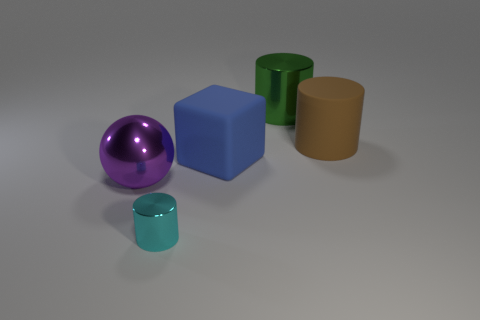
\includegraphics[scale=0.6]{figures/POVQAD中图像示例.png}
\caption{POVQAD中图像示例}
\label{POVQAD-figure}
\end{figure}
\item \textbf{$S_i$}为场景,包含了图像中的所有物体及其属性和位置关系,以JSON格式存储。例如某个场景如下所示:
\begin{lstlisting}
{
  "info": {
    "date": "2025-04-09", // 数据集生成日期
    "split": "training" // 表明当前为训练集
  },
  "image_index": 0, // 图像序号
  "image_filename": "POVQAD_000001.png", // 图像文件名
  "objects": [
    {"shape": "sphere", "color": "red", "size": "large", "material": "rubber", "3d_coords": [1.2, 0.5, 0.3]},
    {"shape": "cube", "color": "blue", "size": "small", "material": "metal", "3d_coords": [-0.5, 1.0, 0.2]},
    {"shape": "cylinder", "color": "green", "size": "medium", "material": "rubber", "3d_coords": [0.0, -1.0, 0.4]}
  ], // 场景中所有物体
  "relationships": {
    "left": [[1], [], [0]],
    "right": [[], [0], [1]],
    "front": [[], [2], [0]],
    "behind": [[2], [], [1]]
  } // 场景中物体之间的空间关系
}
\end{lstlisting}
\item \textbf{$Q_i$}为问题,使用自然语言形式进行表示,例如“What shape is the small red object that is to the left of the yellow cube?”。
每个问题以JSON对象的形式存储在问题文件中,包括问题的自然语言形式、问题对应生成的ASP查询等等。为便于说明,以下是一个问题的样例:
\begin{lstlisting}
{
  "image_filename": "POVQAD_000001.png", // 对应的图像文件名
  "image_index": 1, // 对应的图像的序号
  "question": "What is the color of the cube object?", // 自然语言问题
  "asp_query": "query(Q):-hasProperty(X,color,Q),hasProperty(X,shape,cube).", // ASP查询
  "answer": ["red"], // 答案集
  其余信息此处省略......
}
\end{lstlisting}
问题与对应的场景图像通过图像序号建立联系。
\item \textbf{$\Pi_i$}为环境,是当前图像所属的一组宏观约束规则,采用ASP进行表示。以下为一组约束示例:
\begin{lstlisting}
% 约束示例
% 区域0中所有物体的形状必须是圆柱体
:- obj(X), at(X, 0), has_property(X, shape, cylinder).
% 区域1中蓝色物体的数量大于2个
:- #count{X: has_property(X, color, blue), at(X, 1)} > 2.
\end{lstlisting}
在POVQAD中包含的环境,将在进行积木世界VQA时作为背景知识传递给模型,考察模型利用背景知识进行逻辑推理的能力。
\item \textbf{$A_i$}为答案集,表示该问题对应的正确答案。每个问题的答案和问题一起存储在问题文件中。
\end{enumerate}
\subsection{构建过程}
POVQAD的构建流程如图\ref{fig:dataset-generation}所示,共包括4个步骤。各个步骤的功能如下:
\begin{enumerate}[nosep]
\item \textbf{生成环境}:随机选取部分约束模板,并将模板实例化,最终得到环境。
\item \textbf{构建场景图}:将环境实例化,并将环境输入ASP求解器进行求解,分别生成部分可见场景图和不可见场景图。
\item \textbf{图像渲染}:使用Blender对两类场景图进行渲染,获得积木世界图像与完整的部分可见场景和不可见场景。
\item \textbf{问题生成}:根据问题模板与场景,生成问题与其对应ASP查询,使用Clingo得到问题的答案集并对答案集进行筛选。
\end{enumerate}

最终获得场景文件和问题文件,两者共同组成POVQAD数据集,通过图像编号实现问题文件中的某个问题与其对应场景的匹配。
\begin{figure}[h]
\centering
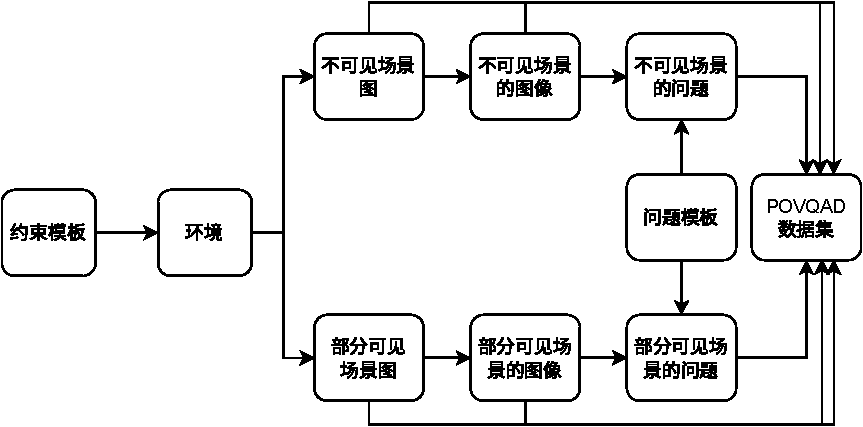
\includegraphics{figures/pipeline-POVQAD-crop.pdf}
\caption{POVQAD构建流程}
\label{fig:dataset-generation}
\end{figure}

\subsubsection{生成环境}
在POVQAD中,一个环境包含了一组约束规则,用于限定在该环境下生成的所有场景所必须满足的
属性组合、区域位置的约束条件。环境的作用是,在宏观层面上对后续生成的图像、问题进行把控,
以控制场景复杂度,并保证数据集保持逻辑一致性。在数学上可以如下表示环境:
$$ \varepsilon = \{C_1,C_2, ..., C_k \}, C_i \in ASP \quad Constraint $$
其中,每个$C_i$是用 ASP 表示的一条逻辑约束规则。

环境的生成过程包括以下步骤:(1)预定义约束模板;(2)确定模板中的相关参数;(3)对所有生成的约束经语义检查与逻辑一致性验证。

此处采用的约束模板与3.2节中所提到的约束模板相同,相关定义在此不再赘述,仅在表\ref{tab:asp_templates}中展示部分模板。
\begin{table}[h]
    \centering
    \renewcommand{\arraystretch}{1.0}
    \begin{tabular}{|p{2.8cm}|p{12.2cm}|}
        \hline
        \textbf{模板} & \textbf{描述} \\
        \hline
        \textbf{模板1(取值约束)} & 
        \texttt{:- obj(X), at(X, R), not has\_property(X, P1, V1).} \\ 
        & 解释: 对区域R中的所有物体,它们P1属性的取值均为V1。 \\ 
        & 具体实现: :- obj(X), at(X, 0), not has\_property(X, color, red). \\
        \hline
        \textbf{模板2(遮挡比例约束)} & 
        \texttt{:- occlusion\_rate(T, R), (R <= 0; R >= 1).} \\ 
        & 解释:物体T被遮挡的比例为R(0<R<=1),完全遮挡时R=1。 \\ 
        & 具体实现::- occlusion\_rate(T, 0.1). \\
        \hline
    \end{tabular}
    \caption{部分约束模板示例}
    \label{tab:asp_templates}
\end{table}

模板实例化生成环境的过程中,需要设定一些参数,具体包括:
\begin{enumerate}[nosep]
\item \textbf{规则模板数量}:每个环境实例化多少条规则模板,默认规定单个环境最多实例化15条。
\item \textbf{属性类型}:将模板中的属性类型占位符用实际生成的属性类型进行替换,例如 P1' 替换为 color,P2' 替换为 shape。
\item \textbf{属性值}:用随机生成的属性值替换,例如 V1' 替换为 red,V2' 替换为 sphere。
\item \textbf{区域范围}:规则作用在哪些区域。根据POVQAD的定义,区域编号为0、1、2、3。
如果是全局作用的模板,则需要将该条规则的作用区域设置为0、1、2、3。如果是作用在局部区域,仅需设置某个或某几个区域即可。
\item \textbf{数量参数}:恰有、至少、至多约束中要求的具体数量。
\end{enumerate}

模板实例化之后,再基于所得的模板实例,为每个区域生成区域内约束,并随机生成跨区域约束和强制否定约束。
强制否定约束用于限制某些属性或者属性做个不能出现在特定区域中,跨区域约束用于限制多个区域之间对象的关系或者属性分布,区域内约束
用于限制单个区域内对象的属性或者属性组合。
最终,得到具体的约束表达式如下所示:
\begin{lstlisting}
:- obj(X), at(X, 0), not hasProperty(X, color, red).
:- obj(X), at(X, 1), hasProperty(X, shape, cube).
:- #count{sameProperty(X1, X2, color): obj(X1), obj(X2), at(X1, 0), at(X2, 1)} < 2.
\end{lstlisting}

POVQAD规定每个环境最多由15条约束规则模板实例化构成,这一数值是经过多方面权衡确定的,目的主要在于以下几方面:
\begin{enumerate}[nosep]
\item 逻辑复杂度与可解性的平衡。如果某个环境中的约束规则过少,会导致后续生成的场景过于松散,
物体属性组合高度自由,推理空间过大,导致问题复杂度过大,难以进行有效推理。
如果约束规则过多,则会造成约束之间产生冲突,导致ASP求解器难以知道合法的解,影响求解效率,进而影响场景的生成。
\item 控制生成时间与可维护性。每条规则在 ASP 中都可能极大影响解空间,规则数上升将显著增加 ASP 求解时间。此外,
在大规模数据生成中,15 条以内的环境可以在数秒内稳定求解出场景,利于批量生成和调试。
\end{enumerate}

此后在生成环境时,将全局约束与获得的约束表达式进行拼接,形成完整ASP程序,并由Clingo对ASP程序进行求解。
如果Clingo的输出至少存在一个答案集,说明当前约束可满足,将所得结果(即环境)保存到ASP程序的\texttt{.lp}文件中。如果Clingo没有答案集,说明当前约束不满足,会
尝试使用其它的约束表达式进行求解,直到能够生成一个环境。

最终,一共生成了30个环境,数据集中的所有场景均匀分布在这些不同的环境之中。
控制生成30个环境的原因是,这一数量的环境实际上可以供后续生成数百万个不同场景和问题,足够支撑进行大规模训练与严格测试。
环境的具体示例见附录\ref{appendix:environment}。
\subsubsection{构建场景}
图\ref{fig:construct-scene}为构建场景的流程图,该流程。
\begin{figure}[h]
\centering
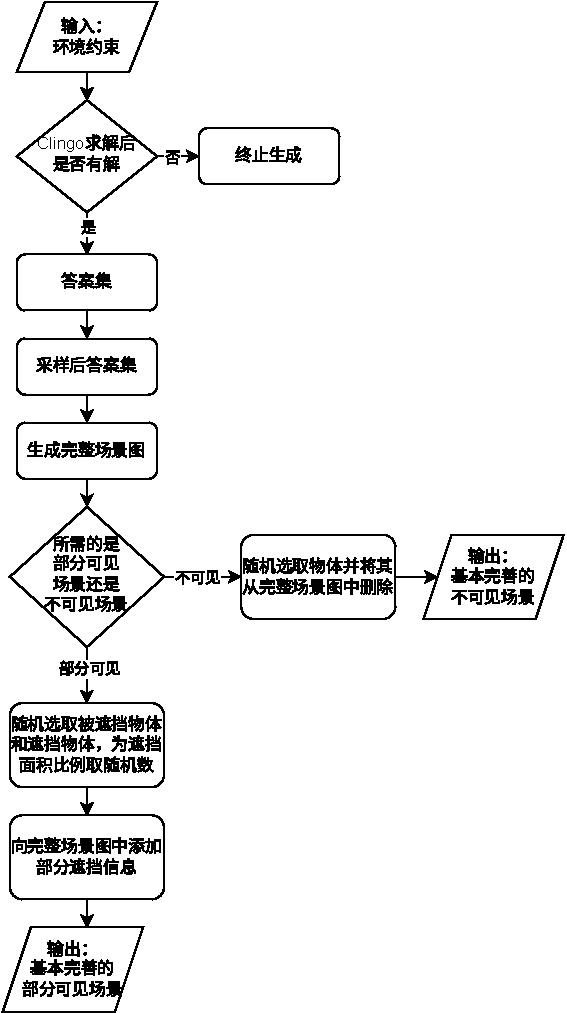
\includegraphics[scale=0.9]{figures/构建场景流程图-crop.pdf}
\caption{构建场景流程图}
\label{fig:construct-scene}
\end{figure}

构建场景的过程中,首先构建完整场景图,此后基于完整场景图分别构造部分可见场景图和不可见场景图,随后基于部分可见场景图和不可见场景图分别构建部分可见场景和不可见场景。
下面本节对构建完整场景图、构建部分可见场景图和不可见场景图分别展开介绍。
\begin{enumerate}[nosep]
\item 构建完整场景图。
在获得环境后,需要进一步获得符合约束的场景图,所需流程为:
将获得的环境约束Clingo进行求解,生成符合约束的答案集,并对答案集进行采样。一个答案集
对应一个完整场景图。此后,将答案集进行解析,获得完整场景图。

首先,将包含了环境约束的\texttt{.lp}文件提交至Clingo进行求解,对Clingo的输出结果进行简单解析,将所有答案集进行提取,此后对答案集进行采样。
在生成答案集之后进行采样出于以下两点原因:
\begin{enumerate}[nosep]
\item 避免处理过多的答案集。如果直接处理所有答案集,会导致后续的场景生成和问题生成过程耗费大量时间和资源。
\item 控制场景的多样性。如果直接使用所有答案集,可能会生成大量相似的场景,导致数据集的多样性不足。
某些约束可能会导致生成的场景具有高度重复的物体属性或关系。随机采样可以增加场景的多样性,避免生成过于相似的场景。
\item 平衡约束类型的答案集。不同的约束类型可能会生成不同数量的答案集。
如果某些约束类型生成的答案集过多,而其他约束类型生成的答案集较少,可能会导致数据集中某些类型的场景占比过高。
对每种约束类型的答案集进行采样,可以平衡不同约束类型的场景数量,确保数据集的均衡性。
\item 降低后续处理的复杂度。每个答案集需要进一步解析为场景图,并用于生成图像和问题。
如果答案集数量过多,会显著增加后续处理的复杂度。通过减少答案集数量,降低后续处理的复杂度,确保生成管道的可控性。
\end{enumerate}

采样之后,对剩余的答案集进行解析处理。对答案集进行解析的过程实际上是对谓词进行解析的过程,
会将\texttt{has\_property}和\texttt{at}两个谓词进行解析,最终形成以JSON格式存储的完整场景图。

场景图是场景的结构化表示,描述了场景中物体的属性以及物体之间的关系,是场景的一种中间表示,
对应场景的\texttt{objects}字段的内容。某个场景图如下所示:
\begin{lstlisting}
{
  0: {"color": "red", "shape": "sphere", "size": "large", "material": "rubber", "region": 0}, // 物体0及其属性
  1: {"color": "blue", "shape": "cube", "size": "small", "material": "metal", "region": 1} // 物体1及其属性
}
\end{lstlisting}

而场景包含了最终渲染的图像及其对应的描述信息,也包括图像中的所有物体及其属性和位置。注意,
只有在最终完成图像渲染时,场景才真正生成完成,才会有\texttt{image\_filename}和\texttt{image\_index}的相关信息,
进行图像渲染之前的场景都是不完整的。

此后基于所得的完整场景可以生成部分可见场景和不可见场景。
\item 构建部分可见场景图。
部分可见场景与完整场景的区别在于:部分可见场景中增加了对于物体之间部分遮挡关系以及遮挡比例的相关信息,进而后续Blender根据场景
渲染图像时,能够得到场景中描述的部分物体之间存在部分遮挡的图像。POVQAD中构建部分可见场景的具体流程如下:

首先从完整场景中,随机选取两个物体,并分别指定一个物体为将会被提问的目标物体\texttt{T}
,另一个物体为去遮挡目标物体的\texttt{Oc}。
此后,向完整场景中添加\texttt{occlusion}字段,用于存放物体间遮挡关系。同时生成一个介于0和1之间的随机数$R$,用于表示目标物体
被遮挡的面积比例。此处为部分可见场景图,$R$应该大于0且小于1,因为当$R=1$时,相当于目标物体被完全遮挡,对应不可见场景的构建,为其它不同的构造方法。
假如此处的$R$取值为0.3,则此时场景的\texttt{occlusion}字段的内容应该为:
\begin{lstlisting}
{
  "occlusion": [
    {T, Oc, 0.3}
  ]
}
\end{lstlisting}
如果场景中不止一对部分遮挡关系,那么继续执行上述流程,直到所有部分遮挡关系添加完毕。
\item 构建不可见场景图。
本环节的目标是,从完整场景图中随机选择一个物体作为被隐藏的目标物体$Obj_i$。
选择目标物体的过程需要满足以下条件:
\begin{enumerate}[nosep]
\item 从完整场景图的所有物体中随机选取一个,在随机选取的过程中,要注意保持均衡,不能
一直选取单一区域的物体或者相同属性的物体,以免造成数据偏态分布。
\item 被选择物体不能是唯一出现某一属性的对象,避免由于移除该物体后,
导致场景图中该属性的值无法被推断,导致问题无解。
\item 该物体将在后续问题中作为查询目标。
\end{enumerate}

选择$Obj_i$后,需要将完整场景图中关于$Obj_i$的所有信息全部移除,生成部分场景。
此时便得到不可见场景图。后续根据不可见场景图可渲染生成不可见场景。
\end{enumerate}
\subsubsection{图像渲染}
图像渲染的目的是依据部分可见场景图以及不可见场景图,使用Blender进行渲染生成图像,生成最终完整的部分可见场景和不可见场景。本环节的具体步骤
在\ref{image-generation}节中已经有过介绍,此处不再赘述。
经过一系列流程之后,最终输出一个JSON对象,其中描述了场景中所有物体之间的空间关系,一个可能的字典如图所示,其中$left[0] = 1$说明
物体0的左侧有物体1,$right[1] = 0$说明物体1的右侧有物体0。
\begin{lstlisting}
{
    "left": [[1], [], [], []],
    "right": [[], [0], [], []],
    "above": [[], [], [3], []],
    "below": [[], [], [], [2]],
    "front": [[1], [], [], []],
    "behind": [[], [0], [], []]
}
\end{lstlisting}
该JSON对象最终作为\texttt{relations}字段的内容,存储到场景中。

在图像渲染完成之后,整个场景构造完成,此时进行数据整合,将所有场景文件合并同一个包含所有场景的JSON文件中。
\subsubsection{问题生成}
图\ref{fig:question-generation}所示为问题生成的流程图。在本环节,POVQAD根据前述步骤整合的场景文件和问题模板来构造自然语言问题。
在POVQAD中,生成的问题均围绕信息缺失物体(在部分可见场景和不可见场景中的目标物体),避免模型通过图像感知直接回答问题,能够更好地考察模型的逻辑推理能力。
一种供参考的模板如\ref{asp:question-template}中所示,
其中<Z1>、<Z2>均表示形状,<C1>、<C2>均表示颜色,<M1>、<M2>均表示材质,<S1>、<S2>均表示尺寸,
<R>表示空间关系。该模板旨在提问具有某种属性的两个物体之间是否处于某种空间位置关系。
这种模板化设计不仅使自然语言问题的结构化描述成为可能,
而且便于后续转换为ASP的形式化表示,从而实现问题求解的自动化。
\begin{lstlisting}[label=asp:question-template]
Is the <Z1> <C1> <M1> <S1> <R> the <Z2> <C2> <M2> <S2>?  
\end{lstlisting}
\begin{figure}[h]
\centering
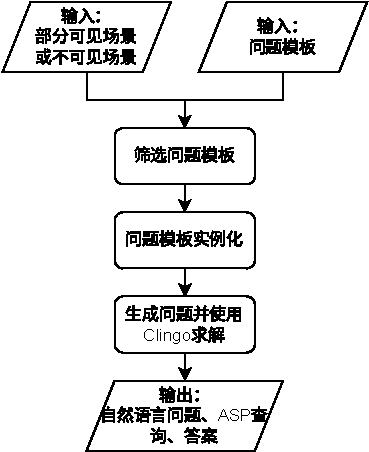
\includegraphics{figures/问题生成-crop.pdf}
\caption{问题生成流程图}
\label{fig:question-generation}
\end{figure}

为全面评估智能体在部分可见积木世界下的空间推理能力,本文设计了三类空间推理问题模板,分别为:位置类问题、位置关系类问题和与位置相关的技术类问题,
分别聚焦不同层次的空间理解与推理要求:
\begin{enumerate}[nosep]
\item 位置类问题用于提问单个目标物体在场景中的具体位置(如“红色立方体在什么位置?”\-),或针对参照物在某一随机方向上的物体属性(如“在绿色圆柱体右侧的物体是什么颜色?”)。
设置该类问题的目的在于检验模型在局部可见性受限时,能否准确识别并定位单一目标。此类问题主要考察视觉感知与属性识别,并验证模型对“部分遮挡”对象的单点推理能力。
\item 位置关系类问题用于询问两个或多个物体之间的空间关系(如“蓝色长方体与黄色圆柱体哪个在前面?”或“哪些物体位于红色立方体的左侧?”)。
设置该类问题的目的在于评测模型在多对象交互下的对称或多元关系推理能力。该类问题要求模型综合考虑多个物体相对位置与遮挡情况,验证其是否能够在部分可见环境中正确构建并推断复杂的空间关系图。
\item 与位置相关的计数类问题则是以某个目标物体为中心,统计满足特定属性或空间条件的邻近物体数量(如“有多少个物体在红色立方体上方?”或“在蓝色圆柱体前方的绿色立方体共有几个?”)。
设置该类问题的目的在于考察模型在定量推理上的表现,尤其是在部分可见和遮挡干扰下对多目标集合的动态筛选与计数能力。此类问题结合了位置关系判断与计数操作,更能反映模型对场景整体结构的理解深度。
\end{enumerate}
通过设置这三类问题,POVQAD不仅能够逐层递进地揭示模型在视觉感知、关系推理与定量计算三方面的短板和强项,还能模拟真实应用场景中常见的“找位置→辨关系→数数量”的操作流程,为神经符号系统
提供了细粒度、可对比的能力评测基准。

具体到问题生成的流程中,首先是筛选问题模板。对模板的筛选,按照模板的查询目标是否与当前场景相匹配,以及模板中给定信息是否在场景中存在来进行。

问题模板筛选完毕之后,根据场景图和筛选好的问题模板,进行模板实例化,生成问题文本及其对应的ASP查询。
实例化过程中,需要对模板中的占位符替换为具体的属性值。对每一个自然语言问题,都是从一个问题模板出发,填充占位符,
然后生成的。所以,自然语言和ASP查询具有一一对应的逻辑结构,可以实现自动转换。

此后调用Clingo求解查询,生成问题的答案,并通过对答案进行分析,实现对生成问题的筛选。
筛选逻辑是:如果答案集为空或者包含所有的可能值,则丢弃当前问题。对生成问题进行筛选有以下三点原因:
\begin{enumerate}[nosep]
\item 提高问题的质量。确保生成的问题有明确的答案,而不是模糊或无意义的问题。
\item 避免冗余问题。避免生成答案集过大的问题,这些问题可能对模型训练没有帮助。
\item 确保问题的多样性。筛选掉覆盖所有可能答案的情况,确保问题具有一定的区分性。
\end{enumerate}

最后,将生成的问题、ASP查询和答案保存为JSON文件,每个问题对应的积木世界图像的名称和序号也会一同记录,为便于说明,此处给出一个样例。
场景文件、各个积木世界图像文件以及此处的问题文件共同构成POVQAD数据集。
\begin{lstlisting}
{
  "split": "train", // 表明当前是训练集
  "image_filename": "POVQAD_000001.png", // 对应的图像文件名
  "image_index": 1, // 对应的图像的序号
  "question": "What is the color of the cube object?", // 自然语言问题
  "asp_query": "query(Q):-hasProperty(X,color,Q),hasProperty(X,shape,cube).", // ASP查询
  "answer": ["red"], // 答案集
  "template_filename": "templates.json", // 使用的问题模板所在的文件
  "question_family_index": 1, // 问题类型序号
  "question_index": 1 // 该问题在其对应类别的问题中的编号
}
\end{lstlisting}
\subsection{数据集质量评估}
为验证构造的POVQAD数据集的可靠性与研究价值,本节从POVQAD的可执行性与一致性、统计分析、对比实验方面进行研究。
\subsubsection{可执行性与一致性评估}
可执行性指的是POVQAD中每个样例的问题对应的ASP程序能够经Clingo求解器执行,不出现语法错误。
一致性指的是对POVQAD中每个样例的问题对应的ASP程序,Clingo对其的求解结果与样例中给出的该问题的标准答案一致。

本文对POVQAD中所有ASP程序依次使用Clingo进行执行,统计语法错误率,结果为0.2\%,
并且对能够正确执行的ASP程序的运行结果与标准答案进行对比分析,一致率为99.5\%,以上两点证明本文生成的ASP程序质量较高,
使用ASP构造POVQAD的方法合理。
\subsubsection{统计分析}
POVQAD中问题分布的统计图见\ref{fig:question_statistics},从图中可以看到位置类问题占比34\%,位置关系类问题占比33\%,
与位置相关的计数类问题占比33\%,总体上实现了三类问题占比1:1:1的要求,做到了问题类型的均匀分布,
这样设计一方面有助于全面评估模型在不同空间推理任务中的能力,避免模型对某一类型问题的过拟合;
另一方面也提升了数据集的科学性和可解释性,使得模型性能对比更加公平合理。
此外,均衡的问题分布也为后续在不同子任务上的研究提供了良好的数据支持基础。
\begin{figure}[h]
    \centering
    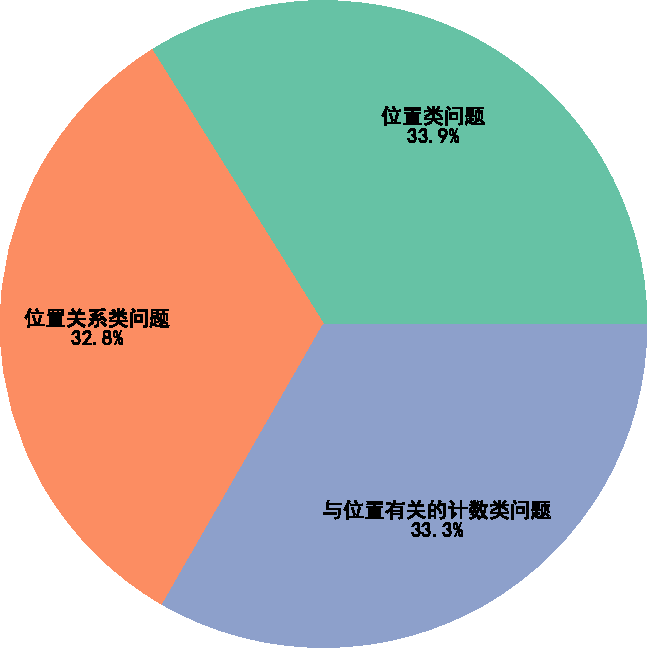
\includegraphics[scale=0.6]{figures/三种类型问题占比-crop.pdf}
    \caption{问题类型分布}
    \label{fig:question_statistics}
\end{figure}
\subsubsection{对比实验}
为了证明POVQAD数据集对不同推理能力方法的区分性与挑战性,
本文选取了五种代表性方法在该数据集上进行实验:传统感知模型(CNN+LSTM)、
主流多模态大模型(DeepSeek、Gemini 2.5 Flash、ChatGPT-4o),以及人类作答作为理论上限参考。
每种方法的输入为POVQAD的图像、自然语言问题以及环境约束。实验重复进行三次取平均值,最终实验结果如图\ref{fig:dataset-comparison}所示,可得出如下结论:
\begin{enumerate}[nosep]
\item 数据集具有良好的难度区分能力。各方法在POVQAD上的准确率差异明显,充分体现了模型间的空间理解与逻辑推理能力差距。尤其是传统模型(CNN+LSTM)仅达到 45.4\% 的准确率,明显低于VLMs方法,显示POVQAD对浅层感知模型构成了挑战。
\item 多模态大模型在不完全信息推理方面存在性能瓶颈。
即便是先进的多模态大模型(如 ChatGPT-4o)也未能达到人类水平,
在复杂场景、信息遮挡和规则约束下的准确率仍有明显提升空间,说明POVQAD能有效考察模型对隐含信息与环境规则的建模能力。
\item POVQAD能作为更强推理任务的评估基准。
结果表明,POVQAD能有效区分浅层感知模型与具备显式推理机制的方法,
同时能检测当前主流多模态模型在空间推理与知识补全方面的能力边界,具备良好的基准测试价值。
\end{enumerate}
\begin{figure}[h]
\centering
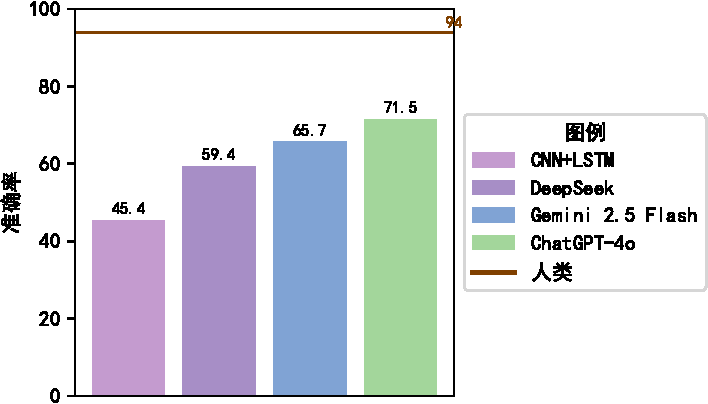
\includegraphics[scale=0.8]{figures/dataset-experiment-crop.pdf}
\caption{不同方法在POVQAD上回答问题的准确率}
\label{fig:dataset-comparison}
\end{figure}
\section{本章小结}
本章聚焦CLEVR数据集的场景完全可见、不要求模型使用外部背景知识进行推理等方面的缺陷,构建一个新的数据集POVQAD,以满足
本文对部分可见积木世界场景下空间推理问答的研究需要。

本章聚焦部分可见积木世界构建任务,从基于ASP的部分可见积木世界构建方法和POVQAD数据集的构建两方面展开介绍,
给出了LLM将自然语言描述的生成指令转化为基于ASP的约束规则的方法,并构造了图像具备部分可见性、问题围绕空间关系展开、考察
模型利用背景知识进行逻辑推理能力的POVQAD数据集,为自动规划课程的教学创新提供了重要依据。

本章也为后续神经符号VQA框架在部分可见积木世界场景下的空间推理问答的实验与分析奠定了坚实的数据基础。